In the following chapter, I will introduce the \ac{PowerTAC} simulation. It's simulating a "liberalized" retail electrical energy market where multiple autonomous agents compete in different markets. Firstly, a retail market where agents, or \emph{brokers}, compete for numerous end-users through the offering of tariff contracts. Secondly, a wholesale market in which brokers buy and sell large amounts of electric energy to match their customers demands. This market allows brokers to place bids up to 24 hours in advance and each hour the broker has the ability to place new bids to correct for changes in their forecast models. Lastly, the balancing market which places relatively high costs on any broker that causes an imbalance in the system, giving incentives to the brokers to balance their own portfolios prior to the balancing operations. Figure ~\ref{fig:powertacoverview} summarizes this ecosystem.
\begin{figure}[!h]%!h
    \centering
    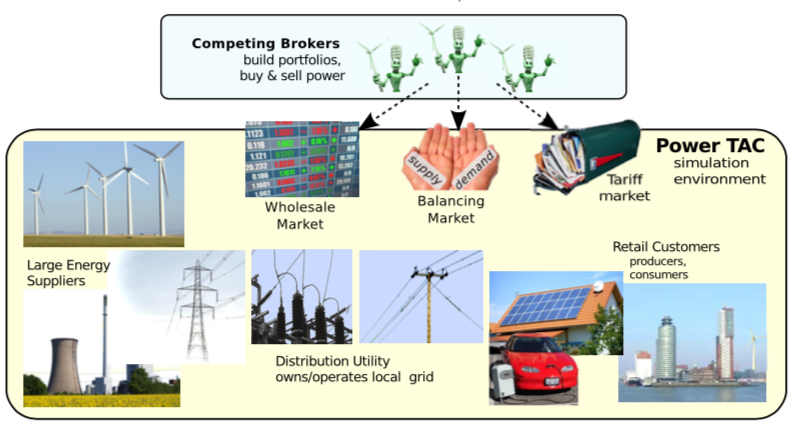
\includegraphics[width=0.9\textwidth]{powerTACScenarioOverview.png}
	\caption{\ac{PowerTAC} overview of markets}
    \label{fig:powertacoverview}
\end{figure}


%OVERVIEW,Economical
The broker to be developed has to contest in a number of markets and handle a variety of customer types. While the \ac{PowerTAC} competition generates a fairly complex landscape, it mostly aims at economic complexity rather than modeling the technical underpinnings of the system. It therefore doesn't simulate any hardware but rather focuses on the different agents involved in the market.

%TIMESLOTS
The simulation emulates a time span of approximately 60 days with 1h time slot precision and accelerates this to 5 real-world seconds corresponding to each game-hour. The simulation emulates a time span of approximately 60 days with 1h time slot precision and accelerates this to 5 real-world seconds corresponding to each game-hour.

\subsection{Components}

The simulation is both technically and logically separated into several components to aid both comprehensibility of the system and yet allow complex simulations of more realistic scenarios. In the following pages, those logical components will be explained. Most of these components are easily mappable into the technical implementation.

\subsubsection{Distribution Utility}
The \ac{DU} represents an entity that regulates the real-time electric usage and corrects for any imbalances in brokers portfolios by correcting the overall net-balance of the system. Any broker who did not balance it's electric supply and demand incurs costs and is therefore incentivized to always balance its portfolios as good as possible. It also owns the distribution grid and every broker must pay fees for the use of the grid in proportion to the number of the customers it serves \citep[p.10]{ketter2018powertac}. It also offers tariffs and is therefore the equivalent of a \emph{baseline broker} whose tariffs create an upper bound on broker profitability. 

\subsubsection{Accounting}
All accounting is managed by the central simulation server as to avoid adversarial brokers from tampering with the games rules. Negative balances are usually punished with a 10\% p.a. interest rate while positive balances receive a 5\% p.a. interest rate. This components tracks every brokers financial balance as well as all brokers customer subscriptions and wholesale market positions \citep[p.11]{ketter2018powertac}.

\subsubsection{Wholesale Market}
%TODO energy or electricity? What's the "right" word? --> ENERGY
Every broker needs to purchase energy before it can sell it to the customers unless the customers of the broker itself generate sufficient energy to balance its own portfolio. For this, \ac{PowerTAC} offers a wholesale market that operates a \emph{periodic double auction} which represents traditional energy exchanges like those existing in the United States and European markets. Participants in this wholesale market are all brokers as well as a large general entity representing a number of generating facilities, a grid buyer who simulates large-scale demands based on real-world data adjusted based on weather-forecasts and a wholesale buyer who regularly places high-volume, low-price bids. During each time slot, 24 future slots are open for placing bids by the brokers. After the bids have been collected, a clearing price gets calculated which is the intersection between the supply and demand curves. Orders without limit prices are always served first. After the clearing, all uncleared bids and asks are distributed to the brokers to indicate the direction of the markets' demand and supply curves. 

\subsubsection{Balancing Market}
The Balancing market is the last and final trading opportunity for agents and in the sense of the game is at $t-0$ meaning that it occurs virtually in parallel to the consume of electricity. Any imbalance during this phase gets corrected for by the \ac{DU} who imposes forced balancing of brokers with an imbalanced portfolio. Brokers with too much supply in their portfolio therefore receive very little reimbursement for it and those whose customers' usage is higher than the estimated amount pay high prices for the additionally supplied energy. 

Brokers who have tariffs with economic control abilities can pass this capacity along to the \ac{DU} who utilizes these capacities to correct the markets imbalances, charging customers' storage devices if an oversupply is present or depleting their devices in the case of an under-supply. It is therefore economically beneficial for brokers to attract customers with such balancing capabilities since it offers a buffer capacity against the balancing costs otherwise incurred through the actions of the \ac{DU} \citep[p.5]{ketter2018powertac} .  





\subsubsection{Customer Market}

The foundation for any broker making profit is a sufficient amount of customers being subscribed to its tariffs. For this to occur, the broker must publish tariffs that are competitive as to attract customers. On the other hand, if the broker offers tariffs that lead to net losses, long term profit will not be possible
\footnote{While the 2017 competition technically allowed for brokers to remain in the game despite offering highly under priced tariffs that corrupted the simulation results, a proper broker must not pursue such strategies simply because of economical reasoning. %TODO verify 2017 corruption
This can be achieved by basing the reward function of the \ac{RL} agent on the financial standing of the agent as reported by the accounting systems of the simulation.}.

The broker has a wide variety of actions at its disposal to create a rich portfolio. The simulation offers the creation of a variety of tariff types that have variables which are adaptable by the broker. The types include:
	
\begin{description}
	\item[Flat rate] Customers pay a flat rate per kWh and they always receive their demanded amount.
	\item[Tariff with fixed fee] Customers pay a definable fixed fee every day to receive the service. 
	\item [Tiered rates] Customers pay a certain price per kWh until a limit is reached after which the kWh price changes. Arbitrarily many such tiers can be added.
	\item[Time-of-use] Customers pay different prices depending on the time of the day or the day of the week.
	\item[Dyanmic Pricing] Allows the broker to dynamically adapt the price per kWh in real-time to incentives customers to reduce their usage during high demand times. A minimum, maximum and mean price per kWh as well as a notification interval needs to be specified. 
	\item[Curtailable] Customers can opt in to a tariff that allows the broker to reduce the delivered amount of electricity per time slot up to a certain percentage. This means the customer is exposed to a risk of not receiving the entire electrical supply demanded, usually for a discounted unit cost per kWh.
	\item[Storage] Customers can offer their storage capacity to brokers to allow the broker to balance his portfolio. Customers receive payment from the broker if their storage devices are being depleted and pay a (reduced) fee for charging events \citep[p.9]{ketter2018powertac}. 
	\item[Signup fees and withdrawl fees] Customers can receive bonuses or pay fees for signing up or canceling a subscription.
\end{description}

Some of the above types can also be combined to create complex tariff landscapes for customers to choose from. 

\subsubsection{Customer models}%
\label{sub:customer_models}

The final part of the simulation environment is made up by the customer models which simulate real-world customers. Each customer can both produce and consume electricity. Consumers are modeled both by factored and elemental models \citep[p.14]{ketter2018powertac}, allowing for small numbers but detailed patterns and large number averaged patterns respectively. The customers evaluate the offered tariffs based on a number of deterministic functions including the various costs and variants of the offered tariffs multiplied by a \emph{irrationality factor} that allows for a more realistic limited rationality of the actors. Additional assessments such as broker reputation evaluation and energy source preferences are also included in the utility function. 

Customers do not evaluate every new tariff but only do so irregularly based on an \emph{inertia factor} that limits their attention to new tariffs. Customers are not inherently loyal to their brokers but the inertia factor indirectly causes customers to not immediately switch if there is a more rational tariff available. 

As previously noted, customers can both consume and produce electricity. While most production is non deterministic and non controllable (i.e. in the case of solar and wind electricity), some are controllable such as \ac{CHP} or bio-gas units \citep[p.16]{ketter2018powertac}. Devices such as electric vehicles or water heaters can also offer regulation actions to brokers to balance their portfolios. A \emph{smart} water heater could refill only minimally after heavy use if usage patterns show that the owners will most likely not use it again for several hours. This way, an additional capacity for energy consumption is created that can be profitable for the customer, as the broker usually charges less for electricity delivered under capacity regulation terms \citep[p.14ff.]{ketter2018powertac}.

\subsection{Broker concepts}
\subsubsection{Decision areas}
\subsubsection{Decision models}
\subsubsection{Past performances}

\subsection{Technology concepts}
\subsubsection{Server technologies}


